\section[Theory]{Theory \textnormal{\cite{GrossMarx+2022}}}
\label{sec:theory}

In the description of condensed matter, tools from classical thermodynamics and statistical physics as well
as quantum mechanical considerations need to be applied. Throughout the following paragraphs, we explore some
of the more well known models in the subfield of thermal properties, specifically for the explanation of the
heat capacity in solids.

\subsection{Heat Capacity}

The heat capacity of any material is defined via
\begin{equation*}
	C \equiv \pfrac{\up{\Delta}Q}{\up{\Delta}T\:}
\end{equation*}
as the amount of heat $\up{\Delta}Q$ corresponding to a unit change $\up{\Delta}T$ in temperature. This is
clearly dependent on the amount of matter, so to allow for comparisons between different materials we can
normalize with volume $V$ or mass $M$ to obtain a specific heat capacity.

\subsubsection{Molar Heat}

In our case, we are interested in the heat capacity per number of particles making up a sample. This leads to
\begin{equation*}
	c \equiv \pfrac{\up{\Delta}Q}{n\up{\Delta}T\:}
\end{equation*}
for the molar heat capacity, where $n$ is the number of \unit{\mole} contained in the substance. To determine
$n$ one can use readily available values of the molar mass $m$ or molar volume $v$ for the given
experimental parameters.

\subsubsection{Measurement}

During the measuring process, it is necessary to constrain certain parameters. To grasp the following relations,
we examine the first and second laws of thermodynamics
\begin{equation*}
	\up{d} U = \up{\delta} Q - \up{\delta} W = T \up{d} S - P \up{d} V
\end{equation*}
where $U$ is the internal energy, $Q$ and $W$ are heat and work, $T$ stands for temperature, $S$ for entropy,
$P$ for pressure and $V$ for volume. The symbols $\up{d}$ and $\up{\delta}$ denote exact and inexact differentials,
respectively. \newpage

From this relation, we identify $\up{\delta} Q = T \up{d} S$ and thereby
\begin{equation*}
	C = T \: \pfrac{\del S}{\del T\:}
\end{equation*}
when translating the defining statement to infinitesimal notation.

\paragraph{Isochoric Case}

At fixed volume, all units of heat result in temperature changes exclusively. The isochoric heat capacity can be written as
\begin{equation*}
	C_V = T \left.\pfrac{\del S}{\del T\:}\right|_V
\end{equation*}
and constitutes an interesting quantity to study the behaviour of materials due to the isolation of otherwise connected effects.

\paragraph{Isobaric Case}

When the pressure is kept constant instead, some of the heat exchange also results in expansion or contraction of the
sample and therefore reduces the total temperature difference. Intuition therefore tells us that $C_P > C_V$ where we write
\begin{equation*}
	C_P = T \left.\pfrac{\del S}{\del T\:}\right|_P
\end{equation*}
for the isobaric heat capacity. This situation is more easily realizable in experiments but comes at the cost of no longer
separating different mechanisms affecting the substance.

\paragraph{Connection}

In order to convert between $C_P$ and $C_V$ we need some generally applicable relationship between the two quantities.
We establish the differential form for entropy
\begin{equation*}
	\up{d}S = \left.\pfrac{\del S}{\del T\:}\right|_V \!\up{d}T + \left.\pfrac{\del S}{\del V\:}\right|_T \!\up{d}V
\end{equation*}
in terms of volume as an extensive and temperature as an intensive property. We obtain
\begin{equation*}
	\left.\pfrac{\del S}{\del T\:}\right|_P \!= \left.\pfrac{\del S}{\del T\:}\right|_V \!+
	\left.\pfrac{\del S}{\del V\:}\right|_T \left.\pfrac{\del V}{\del T\:}\right|_P
\end{equation*}
by differentiating, allowing us to reformulate our desired quantites
\begin{equation*}
	C_P - C_V = T\left(\left.\pfrac{\del S}{\del T\:}\right|_P \!- \left.\pfrac{\del S}{\del T\:}\right|_V \:\right) =
	T\left.\pfrac{\del S}{\del V\:}\right|_T \left.\pfrac{\del V}{\del T\:}\right|_P
\end{equation*}
as the difference between them. \newpage

A combination of Jacobian coordinate transformations and Maxwell relations yields
\begin{equation*}
	C_P - C_V = \alpha_V^2 \, \kappa_T \, TV
\end{equation*}
with the isothermal bulk modulus
\begin{equation*}
	\kappa_T = -V\left.\pfrac{\del P\:}{\del V\:}\right|_T
\end{equation*}
and the volumetric thermal expansion coefficient
\begin{equation*}
	\alpha_V \, = \pfrac{1}{V\:} \left.\pfrac{\del V\:}{\del T\:}\right|_P
\end{equation*}
of the material. For isotropic materials, the last term is equivalent to the form $\alpha_V \, = 3\,\alpha_{\!L}$ via the
linear analogue
\begin{equation*}
	\alpha_{\!L} = \pfrac{1}{L\:} \left.\pfrac{\del L\:}{\del T\:}\right|_P
\end{equation*}
which gives
\begin{equation*}
	C_P - C_V = 9 \, \alpha_{\!L}^2 \, \kappa_T \, TV
\end{equation*}
as the final expression. For typical solids with strong binding forces this difference is negligible, though it becomes
more relevant for liquid or gaseous states of matter.

\subsection{Models}

All approaches discussed in this section model condensed matter as perfect crystal lattices with normal modes of
participating members as purely harmonic oscillations. In the Hooke regime, the center of mass does not change
with increasing or decreasing energy. Accordingly, the volume is constant under heat exchange and the condition
$C_V = C_P$ is always fulfilled. This is of course unphysical, but it should serve as a decent approximation for
the materials we are interested in. To account for thermal contraction, we would need to consider anharmonic
effects by expanding the assumed potential minimum to higher orders.

\subsubsection{Classical Physics}

The equipartition theorem from classical thermodynamics affords a mean energy
\begin{equation*}
	\left< u \right> = \pfrac{1}{2} k_B T
\end{equation*}
to each available degree of freedom. For a singular uncoupled harmonic oscillator, we have the spacial components of
position and velocity as free coordinates. In this view, a three dimensional system of $N$ atoms has an internal energy
\begin{equation*}
	U = 3 N k_B T = 3 nRT
\end{equation*}
when we impose zero equilibrium potential. Here $R = N_{\! A} k_B$ is the universal gas constant, $N_{\! A}$ is the Avogadro
constant and $k_B$ is the Boltzmann constant. \newpage

Because $\up{d}V = 0$ and therefore $\up{d}U = \up{\delta}Q$ we can simply write
\begin{equation*}
	C = \pfrac{\del U}{\del T\:} = 3N k_B = 3nR
\end{equation*}
to find the heat capacity as predicted through the empirical law by Dulong and Petit.

\subsubsection{Quantum Mechanics}

The classical result estimates the heat capacity reasonably well for high temperatures. At lower temperatures however, we
expect quantum mechanical effects to play a significant role. This is explained by the quantization of energy in multiples
of $\hbar\omega$ dividing the range of allowed states into discrete levels. At temperatures where $k_B T \gg \hbar\omega$
the energy space appears continuous to thermal excitations whereas $k_BT \ll \hbar\omega$ forces most members to remain
frozen in the ground state. To visualize this description, figure \ref{fig:quantization} presents a conceptual sketch.

\begin{figure}[H]
	\centering
	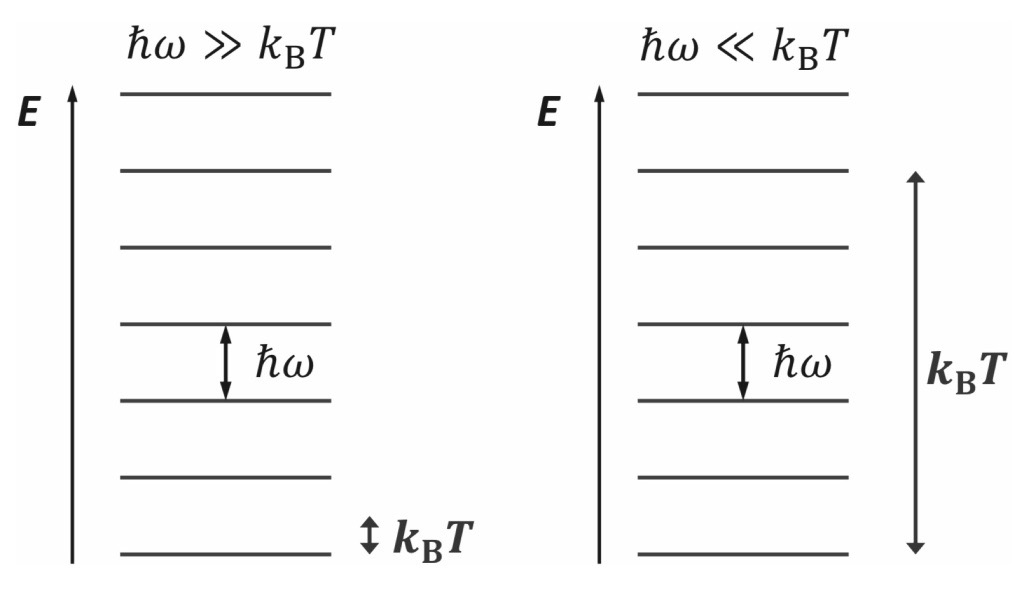
\includegraphics[width=0.4\linewidth]{content/graphics/quantization.jpg}
	\caption{Exemplary energy discretization in low and high temperature limits. \cite{GrossMarx+2022}}
	\label{fig:quantization}
\end{figure}

\paragraph{Phonons}

As shown in figure \ref{fig:branches} collective lattice vibrations show two types of dispersion relation.

\begin{figure}[H]
	\centering
	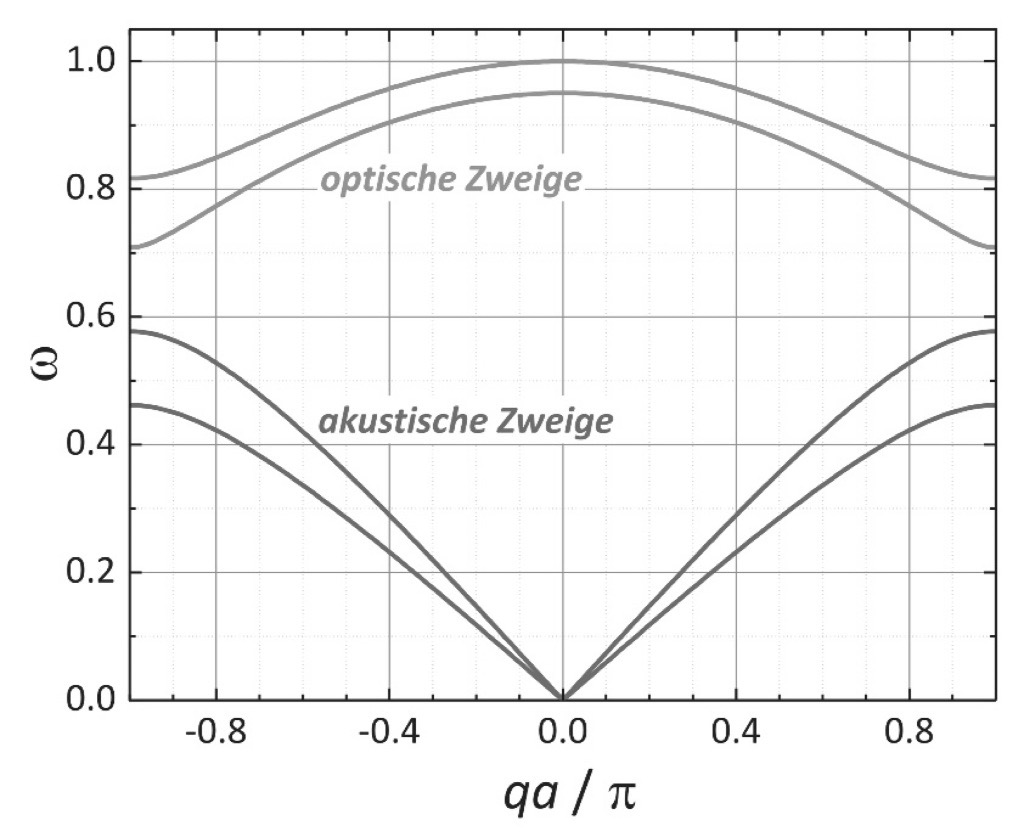
\includegraphics[width=0.45\linewidth]{content/graphics/branches.jpg}
	\caption{Schematic phonon branches inside the first Brillouin zone. \cite{GrossMarx+2022}}
	\label{fig:branches}
\end{figure}

Optical branches result from out of phase oscillations, where neighboring atoms have opposite velocity vectors. Conversely,
acoustic branches represent in phase or parallel vibrational modes. For a crystal with $k$ basis atoms, there are $3$ acoustic
and $3k - 3$ optical dispersion curves. The differences between these solutions can be more or less relevant under different
circumstances.

We call such quantized sound waves phonons, which funtion as quasiparticles with similar behaviour to photons as gauge bosons
acting like quantized light waves. An important characteristic is the vanishing chemical potential $\mu$ indicating
that population numbers are not conserved and that quasiparticles can be created or destroyed.

In accordance with the previous statement, the mean equilibrium population
\begin{equation*}
	\left< n \right> = \pfrac{1}{e^{\beta\hbar\omega} - 1}
\end{equation*}
follows statistics as described by Bose and Einstein, where
\begin{equation*}
	\beta \equiv \pfrac{1}{k_B T\:}
\end{equation*}
is the thermodynamic beta and the exponentials trace back to Boltzmann weighting as well as the convergence of the geometric
series. From the energy levels of a quantum harmonic oscillator
\begin{equation*}
	E_n = \hbar\omega \left( \textstyle{\pfrac{1}{2}} + n \right)
\end{equation*}
we find the internal energy
\begin{equation*}
	U = \sum_{\bm{q}\,r} \textstyle\pfrac{1}{2}\displaystyle \hbar\omega_{\bm{q}\,r} +
	\sum_{\bm{q}\,r} \pfrac{\hbar\omega_{\bm{q}\,r}}{e^{\beta\hbar\omega_{\bm{q}\,r}} - 1}
\end{equation*}
where we sum over all allowed reciprocal vectors $\bm{q}$ and polarisations $r$ to account for multiatomic bases.
The heat capacity follows as
\begin{equation*}
	C = \pfrac{\del}{\del T\:} \sum_{\bm{q}\,r} \pfrac{\hbar\omega_{\bm{q}\,r}}{e^{\beta\hbar\omega_{\bm{q}\,r}} - 1}
\end{equation*}
in the most general case. Due to $\sum_{\bm{q}\,r} = 3N$ we always get $C = 3Nk_B$ at high temperatures
by expanding the exponential function to linear order. This asymptote reproduces the classical result as asserted by
the correspondence principle independent from any further restrictions introduced by additional simplifications. The global
models described below therefore both approach the same value at high thermal energies but differ when quantum effects
dominate at low temperatures. \newpage

\paragraph{Einstein}

The core assumption proposed by Einstein is a monochromatic eigenmode spectrum. By introducing $\omega_E$ as the
frequency for all oscillations, we can write
\begin{equation*}
	C = \pfrac{\del}{\del T\:} \sum_{\bm{q}\,r} \pfrac{\hbar\omega_E}{e^{\beta\hbar\omega_E} - 1}
\end{equation*}
and after differentiating
\begin{equation*}
	C = 3N \, \pfrac{\hbar^2 \omega_E^2}{k_B T^2} \, \pfrac{e^{\beta\hbar\omega_E}}{( e^{\beta\hbar\omega_E} - 1 )^2}
\end{equation*}
with $\sum_{\bm{q}\,r} = 3N$ for the summation. We introduce the Einstein temperature
\begin{equation*}
	\vartheta_{\! E} \equiv \pfrac{\hbar\omega_E}{k_B}
\end{equation*}
and reformulate the previous expression as
\begin{equation*}
	C = 3N k_B \, \Bigl(\pfrac{\vartheta_{\! E}}{T}\Bigr)^{\!\! 2} \pfrac{e^{\vartheta_{\! E} / T}}{( e^{\vartheta_{\! E} / T} - 1 )^2}
\end{equation*}
for our result. By using the expansions $e^{\vartheta_{\! E} / T} = 1$ and $e^{\vartheta_{\! E} / T} - 1 = \vartheta_{\! E} / T$
it is trivial to show that $C = 3N k_B$ at high temperatures. With $e^{\vartheta_{\! E} / T} \gg 1$ we find
\begin{equation*}
	C = 3N k_B \, \Bigl(\pfrac{\vartheta_{\! E}}{T\:}\Bigr)^{\!\! 2} e^{-\vartheta_{\! E} / T}
\end{equation*}
in the low temperature limit. The flat dispersion underlying these results most closely resembles the typical behavior
of optical phonons. Due to their contribution being most significant at higher energies, the accuracy of the cold regime
approximation suffers as acoustic phonons dominate.

\paragraph{Debye}

According to Debye, we replace all phonon branches with the three acoustic ones and approximate these to exhibit linear
dispersion. Additionally, instead of summing over wave vectors $\bm{q}$ we integrate over a spherical constant energy
surface of the first Brillouin zone. Each dispersion branch contains $N$ states occupying a total phase space
volume
\begin{equation*}
	8\pi^3 \pfrac{N}{V\:} = \pfrac{4}{3} \pi q_D^3
\end{equation*}
where the right hand side follows as the volume of a sphere with radius $q_D$ equal to the magnitude of the reciprocal
Debye vector. \newpage

Solving this equation leads to
\begin{equation*}
	q_D = \left( 6\pi^2 \pfrac{N}{V\:} \: \right)^{\!\!1/3}
\end{equation*}
which defines $\omega_{D\,i} = q_D v_i$ for the frequencies. We see here that the speed of sound
\begin{equation*}
	v_i = \frac{\omega_{D\,i}}{\raisebox{0.25ex}{$q_D$}} = \frac{\del \omega_{D\,i}}{\del q_D}
\end{equation*}
is both the phase and group velocity. Accounting for the density of states, we find
\begin{equation*}
	C = \,\pfrac{\del}{\del T\:} \sum_{i = 1}^3 \int_0^{2\pi} \up{d} \varphi
	\int_0^\pi \up{d}\vartheta \sin\vartheta \int_0^{q_D} \up{d}q \,q^2 Z(q) \,\pfrac{\hbar q v_i}{e^{\beta\hbar q v_i} - 1}
\end{equation*}
in spherical coordinates. We define the cubed harmonic mean sound velocity $v_s$ via
\begin{equation*}
	\pfrac{1}{v_{\! s}^3} = \pfrac{1}{3} \sum_{i=1}^3 \pfrac{1}{v_i^3}
\end{equation*}
or more explicitly
\begin{equation*}
	v_{\! s} = \Bigl( \raisebox{0.25ex}{$\displaystyle\pfrac{1}{3v_l^3} + \pfrac{2}{3v_t^3}$} \Bigr)^{\!\! -1/3}
\end{equation*}
where we require identical velocities $v_t$ for both transversal components with the singular longitudinal mode $v_l$ as independent.
Using this, we can write
\begin{equation*}
	C = \pfrac{3V\hbar^2 v_{\! s}^2}{2\pi^2k_B T^2} \int_0^{q_D} \up{d}q \,
	\pfrac{q^4 e^{\beta\hbar q v_{\! s}}}{(e^{\beta\hbar q v_{\! s}} - 1)^2}
\end{equation*}
after integrating over the solid angle and differentiating with respect to temperature. The substitution
$x \equiv \beta\hbar q v_{\! s}$ gives
\begin{equation*}
	C = \pfrac{3V k_B^4 T^3}{2\pi^2 \hbar^3 v_{\! s}^3} \int_0^{\beta\hbar q_D v_{\! s}} \up{d}x \, \pfrac{x^4 e^x}{(e^x - 1)^2}
\end{equation*}
as an equivalent formulation. By introducing the Debye temperature
\begin{equation*}
	\vartheta_{\! D} \equiv \pfrac{\hbar\omega_D}{k_B} = \pfrac{\hbar q_D v_{\! s}}{k_B} = \pfrac{\hbar v_{\! s}}{\k_B}
	\left( 6\pi^2 \pfrac{N}{V\:} \: \right)^{\!\!1/3}
\end{equation*}
we finally arrive at
\begin{equation*}
	C = 9N k_B \Bigl( \pfrac{T}{\vartheta_{\! D}} \Bigr)^{\! 3} \int_0^{\vartheta_{\! D} / T} \up{d}x \, \pfrac{x^4 e^x}{(e^x - 1)^2}
\end{equation*}
for our result. At high temperatures $e^x = 1$ and $e^x - 1 = x$ lead to $C = 3N k_B$ again. \newpage

In the case of low temperatures, the integral approaches
\begin{equation*}
	\int_0^\infty \up{d}x \, \pfrac{x^4 e^x}{(e^x - 1)^2} = \pfrac{4\pi^4}{15}
\end{equation*}
and the heat capacity
\begin{equation*}
	C = \pfrac{12\pi^4}{5} N k_B \Bigl( \pfrac{T}{\vartheta_{\! D}} \Bigr)^{\! 3}
\end{equation*}
has a cubic temperature dependence. Thanks to the assumption of linear dispersion, this closely matches observations.
From the above considerations
\begin{equation*}
	\omega_D = q_D v_{\! s} = \left( 18\pi^2
	\Bigl( \raisebox{0.25ex}{$\displaystyle\pfrac{1}{v_l^3} + \pfrac{2}{v_t^3}$} \Bigr)^{\!\! -1}
	\pfrac{N}{V\:} \: \right)^{\!\!\! 1/3} 
\end{equation*}
gives the prescription for the resulting frequency.

\paragraph{Electrons}

Especially in metals, the contribution from free electrons can add significantly to the heat capacity. We model this as an
ideal fermion gas, meaning that all interactions are governed by the Pauli exclusion principle, resulting in a statistic
as described by Fermi and Dirac. From a Sommerfeld expansion we find
\begin{equation*}
	C = \pfrac{\pi^2}{2} N k_B \pfrac{T}{T_F\,}
\end{equation*}
where the Fermi temperature $T_F$ is defined via the Fermi energy $E_F = k_B T_F$ and the heat capacity depends linearly
on the absolute temperature. Exemplary isochoric heat capacities can be viewed in figure \ref{fig:comparison} to compare
the competing models.

\begin{figure}[H]
	\centering
	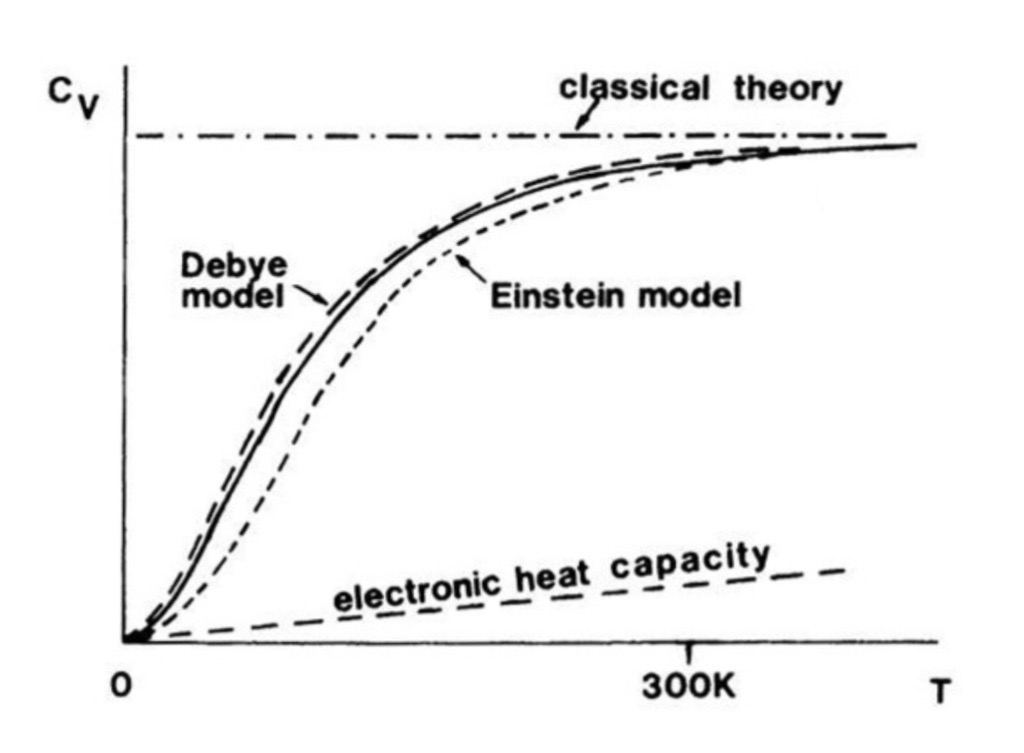
\includegraphics[width=0.5\linewidth]{content/graphics/comparison.jpg}
	\caption{Different models of isochoric heat capacity for a typical solid material. \cite{what-when-how}}
	\label{fig:comparison}
\end{figure}
